%!TEX root = templateICI.tex
%!TEX spellcheck=es_ES

\chapter{Diseño}\label{ch:Diseno}

\section{Diseño Arquitectónico}\label{sc:DA}
    \subsection{Tecnologías utilizadas}\label{ssc:tech}
    En esta sección se detallaran las tecnologías a utilizar para optimizar el código del prototipo,
    para poder analizar el código (segunda etapa de la metodología a utilizar), la herramienta AutoPerf
    sera la utilizada en su ultima versión.
    Autoperf es una herramienta para crear y administrar experimentos de rendimiento, incluido el procesamiento y análisis de datos.
    Proporciona un formato simple para definir el entorno del experimento y los datos que se recopilarán, e interactúa con una variedad de herramientas de rendimiento. Junto con lo anterior, la herramienta  HPCToolkit es un conjunto integrado de herramientas para medir y analizar el rendimiento del programa en computadoras que van desde sistemas de escritorio multinúcleo a las supercomputadoras más grandes del país.
    Al utilizar un muestreo estadístico de temporizadores y contadores de rendimiento de hardware, HPCToolkit recopila mediciones precisas del trabajo, el consumo de recursos y la ineficiencia de un programa y las atribuye al contexto de llamada completo en el que se producen. HPCToolkit funciona con aplicaciones que están vinculadas estática o dinámicamente.
    Dado que HPCToolkit utiliza el muestreo, la medición tiene una sobrecarga baja (1-5\%) y se escala a grandes sistemas paralelos. Las herramientas de presentación de HPCToolkit permiten un análisis rápido de los costos de ejecución, ineficiencia y características de escalamiento de un programa tanto dentro como a través de los nodos de un sistema paralelo. HPCToolkit admite la medición y el análisis de códigos de serie, códigos de subprocesos (por ejemplo, pthreads, OpenMP), MPI y códigos paralelos híbridos (subprocesos de MPI +).

    En la etapa de Realizar Modificaciones se utilizara LIBXSMM que es una biblioteca para operaciones especializadas de matriz densa y dispersa, dirigidas a la arquitectura Intel. Los núcleos de multiplicación de matriz pequeña (SMM) se generan para Intel SSE, Intel AVX, Intel AVX2, IMCI (KNCni) para coprocesadores Intel Xeon Phi (KNC), e Intel AVX-512 tal como se encuentran en la familia de procesadores Intel Xeon Phi (KNL, KNM). ) y procesadores Intel Xeon (SKX).
    La biblioteca es compatible con el código generado de manera estática en el momento de la configuración (SMM), utiliza rutas de código optimizadas basadas en el código generado por el compilador, así como en las funciones intrínsecas, pero utiliza principalmente la especialización de código Just-In-Time (JIT) para el rendimiento independiente del compilador (multiplicaciones de matrices). , matriz de transposición / copia, funcionalidad dispersa y pequeñas circunvoluciones). LIBXSMM es adecuado para "compilar una vez e implementar en todas partes", es decir, no se necesitan indicadores de destino especiales para explotar el rendimiento disponible.
    En la tabla \ref{tab:tool} detalla las herramientas a utilizar junto con las etapas y paginas oficiales.

\begin{table}
    \begin{tabular}{|l|l|l|}
\hline
        Herramienta  & Etapa                   & Dirección Web                    \\ \hline
        HPCToolkit & Análisis de Código      & http://hpctoolkit.org/           \\
        AutoPerf   & Análisis de Código      & https://github.com/HPCL/autoperf \\
        LIBXSSM    & Realizar Modificaciones & https://github.com/hfp/libxsmm  
    \end{tabular}
    \caption{Tabla Herramientas a Utilizar.}
    \label{tab:tool}
\end{table}



    \subsection{Flujo de datos / Vista de alto nivel}\label{ssc:flow}



\section{Diseño Lógico}\label{sc:DL}
    \subsection{Diagrama de despliegue}\label{ssc:diagDesp}
    Los diagramas de despliegue (DD) se utilizan para visualizar los detalles de implementación de un sistema de software. Los diagramas incluyen más que sólo código, sino también bibliotecas separadas, un instalador, archivos de configuración y muchas otras piezas. Para que el software esté listo para ejecutarse, es necesario comprender todos los archivos y ejecutables involucrados y los entornos donde residen.

    El DD Ilustra el hardware del sistema y su software. Útil cuando se implementa una solución de software en múltiples máquinas con configuraciones únicas.

    Dos tipos especiales de dependencias: la importación de paquetes y la fusión de paquetes.

    Pueden representar los diferentes niveles de un sistema para revelar la arquitectura. Deben indicar las dependencias entre paquetes y comunicación entre estos.

    En la Figura~\ref{fig:DD}, se presenta un ejemplo de un diagrama de despliegue.

    \begin{figure}[H]
        \centering
        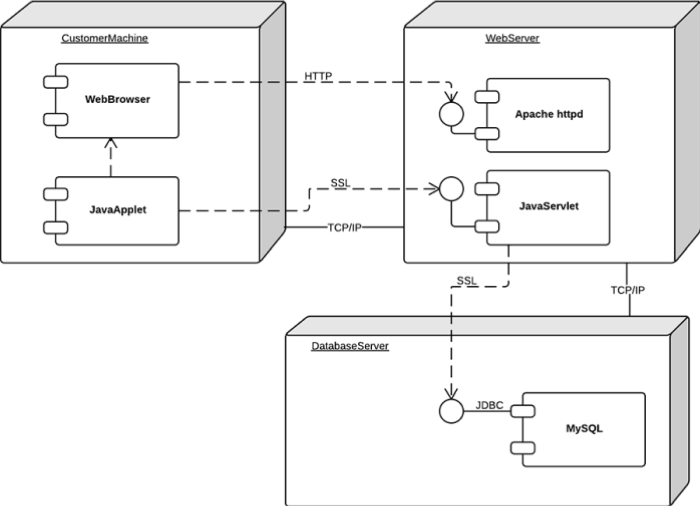
\includegraphics{imagenes/DD.png}
        \caption{Ejemplo Diagrama de Despliegue}
        \label{fig:DD}
    \end{figure}




    \subsection{Diagrama de componentes}\label{ssc:diaComp}
    En esta sección se explicara el diagrama de componentes del sistema, el componente paciente carga los datos desde el componente de Persistencia.
    El primero carga los datos en el Controlador que entrega datos a la Interfaz.
    Los datos son obtenidos desde el componente Captura Datos, que el componente Medicion se los entrega al modulo DSP.
    Finalmente, los diagramas de componentes pueden ilustrar una relación de dependencia. Una relación de dependencia ocurre cuando la interfaz provista por un componente coincide con la interfaz requerida por otro componente. La interfaz proporcionada está representada por una bola, y la interfaz requerida está representada por un \textit{socket}.

      A continuación, en la figura~\ref{fig:componentDiagram}, se presenta el diagrama de componentes para el prototipo:

        \begin{figure}[H]
        \centering
        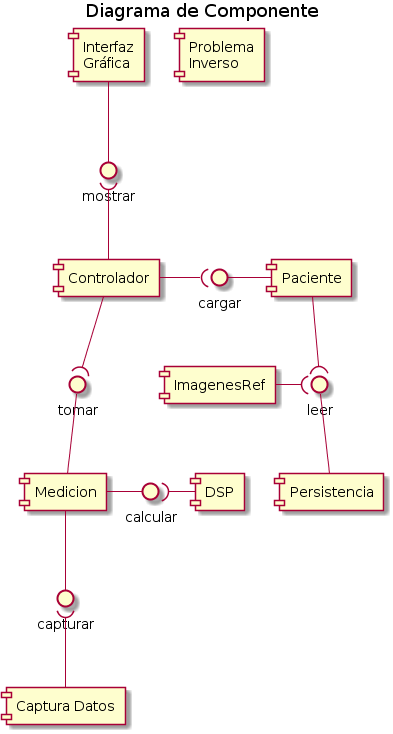
\includegraphics[width=0.7\linewidth]{imagenes/componentDiagram.png}
        \caption{Diagrama de Componentes}
        \label{fig:componentDiagram}
    \end{figure}

    Los diagramas de componentes son especialmente útiles al principio del proceso de diseño, debido a su énfasis de alto nivel. Se pueden realizar en diferentes niveles y le permiten enfocarse no sólo en los sistemas sino también en los subsistemas.


    \subsection{Diagrama de paquetes}\label{ssc:pack}

    Los diagramas de paquetes muestran los paquetes y las dependencias entre ellos. Estos diagramas pueden organizar un sistema completo en paquetes de elementos relacionados, estos podrían incluir datos, clases o incluso otros paquetes. Los diagramas de paquetes ayudan a proporcionar agrupaciones de alto nivel de un sistema para que sea fácil visualizar cómo un paquete contiene elementos relacionados, así como la forma en que los diferentes paquetes dependen entre sí.

    A continuación, en la figura~\ref{fig:packageDiagram}, se presenta un ejemplo de un diagrama de paquetes para un videojuego:

    \begin{figure}[H]
        \centering
        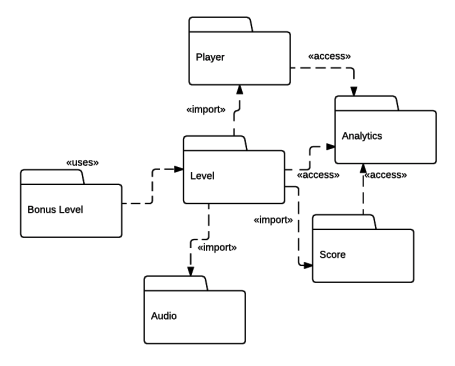
\includegraphics[width=0.7\linewidth]{imagenes/packageDiagram.png}
        \caption{Ejemplo Diagrama de Paquetes}
        \label{fig:packageDiagram}
    \end{figure}

    \subsection{Diagrama de clases}\label{ssc:clases}

El Diagrama de clase da la vista estática de una aplicación. Un diagrama de clase describe los tipos de objetos en el sistema y los diferentes tipos de relaciones que existen entre ellos. Este método de modelado se puede ejecutar con casi todos los métodos orientados a objetos.

El Diagrama de clase ofrece una descripción general de un sistema de software al mostrar clases, atributos, operaciones y sus relaciones. Este diagrama incluye el nombre de la clase, los atributos y la operación en compartimientos designados separados.

Para finalizar, el Diagrama de clase ayuda a construir el código para el desarrollo de aplicaciones de software.

Los elementos esenciales en un diagrama de clases son:

\begin{itemize}
    \item Nombre de la clase
    \item Atributos
    \item Operaciones
\end{itemize}

A continuación, en la figura~\ref{fig:classesDiagram}, se presenta un ejemplo de un diagrama de clases:
    \begin{figure}[H]
        \centering
        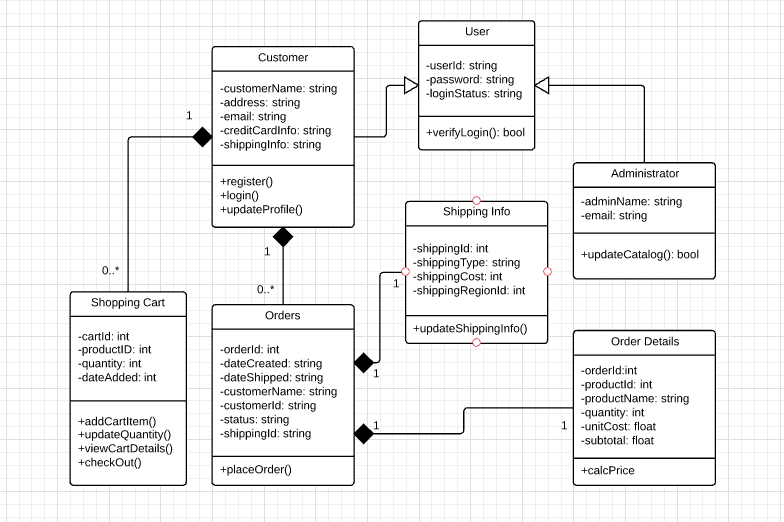
\includegraphics[width=0.7\linewidth]{imagenes/classesDiagram.png}
        \caption{Ejemplo Diagrama de Clases}
        \label{fig:classesDiagram}
    \end{figure}


\section{Diseño de Datos}\label{sc:DD}
    \subsection{Diagrama Entidad Relación}\label{ssc:ER}
    \subsection{Diagrama Relacional}\label{ssc:Rel}
    \subsection{Diccionario de Datos}\label{ssc:DD}

\section{Diseño de Interfaz}\label{sc:DI}
    \subsection{Arquitectura de la Información}\label{ssc:AA}
    \subsection{Prototipos de Interfaces Gráficas}\label{ssc:IGraph}
    %\subsection{}\label{ssc:}

\section{Diseño de Pruebas}\label{sc:DP}
    \subsection{Pruebas Unitarias}\label{ssc:UT}
    \subsection{Pruebas de Integración}\label{ssc:IT}
    \subsection{Pruebas con Usuarios}\label{ssc:PU}
    \subsection{Pruebas de Aceptación}\label{ssc:PA}

\section{Diagramas Opcionales / Complementario}\label{sc:OP}
    \subsection{Diagramas de Actividad}\label{ssc:DA}
